\documentclass[12pt]{article}
\usepackage{amsmath, graphicx, caption}
\usepackage{amsthm}
\usepackage{amsfonts, xcolor, physics}
\usepackage{amssymb}
\usepackage{mathrsfs}
\usepackage[T1]{fontenc} % for \symbol{92} 
\usepackage{comment, subfig, hyperref, url}


\addtolength{\oddsidemargin}{-1in}
\addtolength{\evensidemargin}{-1in}
\addtolength{\textwidth}{1.75in}
\addtolength{\topmargin}{-1in}
\addtolength{\textheight}{1.75in}
\newcommand{\contra}{$\rightarrow\leftarrow$}
\newcommand{\tb}{  \textbackslash  }
\newcommand{\bj}{\ \Longleftrightarrow \ }

%bailey meche
\begin{document}
%bailey meche
	\begin{center}
		ECMA 31140: Perspectives on Computational Modeling for Economics\\
        Problem Set 1\\
		Due Date: January 14th, 2025 \\
        Bailey Meche
	\end{center}

\emph{Solution code can be found at the following GitHub repository:} \href{https://github.com/BaileyMeche/macs30150_Winter25}{MACS 30150 Repo}

\section*{Instructions}

You are encouraged to work and discuss in groups, but you must submit your work individually. Answers must be legibly hand-written or typed. All assignments are due electronically on Canvas. Attach your code. Assignments are due at \textbf{12:30 PM}. Late problem sets will not be accepted.



\section*{Problem 1: The Zero of an Arbitrary Function (30 points)}

Consider the following function:
\[
f(x) = (x - 10)e^{-x^2} + 5
\]
The objective is to find the zero of the function, that is, the value \(x^*\) such that \(f(x^*) = 0\). Restrict the problem to finding solutions for positive values of \(x\).

\begin{enumerate}
    \item[(a)] Write up a code yourself to find the zero of the function implementing the {Bisection method}. (15 points)

    \textbf{Solution}

    Zeroes of the function are $[-0.8818,    0.7821]$. Code can be found at \url{macs_pset1_1a.m}.

    
    \item[(b)] Write up a code yourself to find the zero of the function implementing the {Newton-Raphson method}. Consider different starting values. Assess how reliable this algorithm is in finding the solution. Is the Bisection method better? Discuss. (15 points)

    \textbf{Solution}

    Zeroes of the function are $[-0.8818,    0.7821]$. Code can be found at \url{macs_pset1_1b.m}.
    
\end{enumerate}

\section*{Problem 2: Equilibrium Interest Rate (50 points)}

Assume two large groups of individuals (each of the same unit mass or measure). They are identical within the group but different between groups. Let \(j = a, b\) index individuals of type \(a\) and \(b\) respectively. Each lives only two periods and they have endowments in each period as follows:
\[
y_{i0}^j = y_0, \quad y_{i1}^j = y_1, \quad \text{with } 2y_0 = y_1.
\]
They maximize:
\[
\sum_{t=0}^{1} \beta^t u_j(c_{it}^j),
\]
subject to:
\[
c_{i0}^j + b_i^j = y_0, \quad c_{i1}^j = y_1 + b_i^j(1 + r),
\]
where \(r\) is the real interest rate. Assume:
\[
u_a(c_{it}^a) = \frac{(c_{it}^a)^{1-\sigma_a}}{1-\sigma_a}, \quad u_b(c_{it}^b) = \frac{(c_{it}^b)^{1-\sigma_b}}{1-\sigma_b}, \quad \beta = 0.95.
\]

\begin{enumerate}
    \item[(a)] Define the Competitive Equilibrium of the Economy. (10 points)

    \textbf{Solution}

 Each household $j=a,b$ chooses consumption and savings to maximize lifetime utility
 \begin{equation}\label{max}
     \max_{c_{i0}^j, c_{i1}^j, b_i^j} \sum_{t=0}^{1} \beta^t u_j(c_{it}^j) = \max_{c_{i0}^j, c_{i1}^j, b_i^j} \left\{ u_j(c_{i0}^j) + \beta u_j(c_{i1}^j)   \right\} 
 \end{equation}
    subject to the constraints 
    \[
c_{i0}^j + b_i^j = y_0, \quad c_{i1}^j = y_1 + b_i^j(1 + r).
\]
Using the utility functions $u_a(c_{it}^a)$ and $u_b(c_{it}^b),$ the marginal utilities are 
\[ \frac{\partial }{\partial c_{it}^a}u_a(c_{it}^a) = (c_{it}^a)^{-\sigma_a}, \quad \frac{\partial}{\partial c_{it}^b}  u_b(c_{it}^b) = (c_{it}^b)^{-\sigma_b} \]
    The Lagrangian for \eqref{max} is then 
    \[
\mathcal{L}_b = \frac{(c_{i0}^b)^{1-\sigma_b}}{1-\sigma_b} + \beta \frac{(c_{i1}^b)^{1-\sigma_b}}{1-\sigma_b} + \lambda_b \left(y_0 - c_{i0}^b - b_i^b\right) + \mu_b \left(y_1 + b_i^b(1 + r) - c_{i1}^b\right).
\]

The First-Order Conditions for household Type $b$:
\begin{enumerate}
    \item $\frac{\partial \mathcal{L}_b}{\partial c_{i0}^b} = (c_{i0}^b)^{-\sigma_b} - \lambda_b = 0 ; \quad  \lambda_b = (c_{i0}^b)^{-\sigma_b}$
    \item $\frac{\partial \mathcal{L}_b}{\partial c_{i1}^b} = \beta (c_{i1}^b)^{-\sigma_b} - \mu_b = 0 ; \quad  \mu_b = \beta (c_{i1}^b)^{-\sigma_b}$
    \item $\frac{\partial \mathcal{L}_b}{\partial b_i^b} = \lambda_b - \mu_b(1 + r) = 0 ; \quad  \lambda_b = \mu_b (1 + r)$
    \item Budget constraints: $c_{i0}^b + b_i^b = y_0, \quad c_{i1}^b = y_1 + b_i^b(1 + r)$
\end{enumerate}

From (c) and substituting in (a) and (b):
\[
\lambda_b = \mu_b (1+r) \quad \implies_{(a),(b)} \quad (c_{i0}^b)^{-\sigma_b} = \beta (1 + r) (c_{i1}^b)^{-\sigma_b}.
\]

The bond market clears at 
\[
b_i^a + b_i^b = 0.
\]
Using the budget constraints, we have 
\[
b_i^j = y_0 - c_{i0}^j%, \quad b_i^b = y_0 - c_{i0}^b.
\]

Substitute into the market clearing condition:
\[
y_0 - c_{i0}^a + y_0 - c_{i0}^b = 0 \implies c_{i0}^a + c_{i0}^b = 2y_0, \ c_{i1}^a + c_{i1}^b = 2y_1
\]

Therefore, the competitive equilibrium consists of  allocations $(c_{i0}^a, c_{i1}^a, c_{i0}^b, c_{i1}^b, b_i^a, b_i^b)$ and a real interest rate \(r\)
such that:
\begin{enumerate}
    \item Budget constraints 
    \[ c_{i1}^j = y_1 + (y_0 - c_{i0}^j)(1 + r) \]
    \item  The bond market clears at 
\[
c_{i0}^a + c_{i0}^b = 2y_0
\]
\item The first-order conditions are satisfied:
\[
(c_{i0}^a)^{-\sigma_a} = \beta (1 + r) (c_{i1}^a)^{-\sigma_a}, \quad (c_{i0}^b)^{-\sigma_b} = \beta (1 + r) (c_{i1}^b)^{-\sigma_b}.
\]
\item Numerical solution from \verb!macs_pset1_2a.m! provides that 
\[(c_{i0}^a, c_{i1}^a, c_{i0}^b, c_{i1}^b, b_i^a, b_i^b, r) = (0.9633, 2.2015, 1.0367 , 1.7985,0.0367, -0.0367,  4.4971) \]


\end{enumerate}

This indicates that for $\sigma_a =2, \sigma_b=3$ and given endowments, we have the following interpretations. 

Households Type $a$ consumes slightly less than half of their period 0 endowment, and save part of their period 0 endowment to enjoy higher consumption in period 1.
Households Type $b$ consumes slightly more than half of their period 0 endowment, and borrow in period 0 and consumes less in period 1 to repay the bond. Total consumption in period 0 satisfies the market clearing condition $c_{i0}^a + c_{i0}^b = 2y_0 =2$. The equilibrium interest rate is approximately 450\%. This high interest rate arises because type $b$ has a higher risk aversion $(\sigma_b > \sigma a)$, leading to a strong borrowing motive balanced by the savings from type $a$.

    \bigskip 
    %%%%%%%%%%%%%%%%%%%%%%%%%%%
    \item[(b)] Find the equilibrium \(r\) for each combination of \(\sigma_a, \sigma_b\), where each belongs to a set of evenly spaced values starting at 0.1 and ending at 2, with size 100. (20 points)

    \textbf{Solution}

    The Matlab code for the solution below is found at \verb!macs_pset1_2b.m! and the values themselves are found at \verb!macs_pset1_2b_results.csv!.
    
\begin{figure}[h!]
    \centering
    % First image for Type a
    \begin{minipage}{0.45\textwidth}
        \centering
        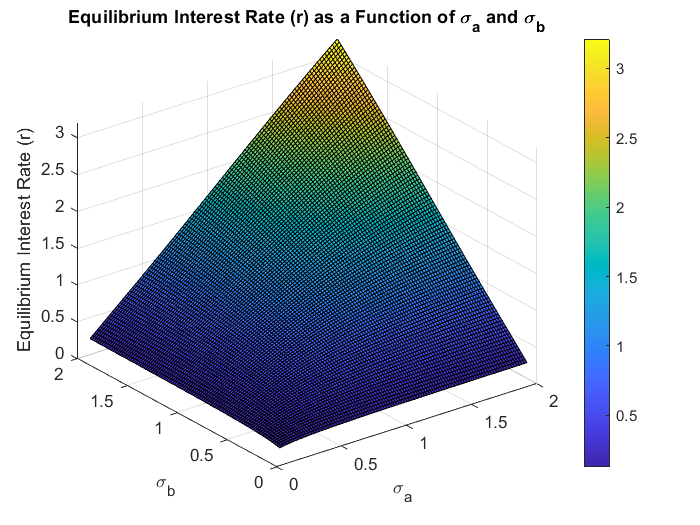
\includegraphics[width=\textwidth]{2b_2.png}
        \caption{Equilibrium Interest Rate $r$ as a Function of $\sigma_a, \sigma_b$.}
        \label{fig:2b_2}
    \end{minipage}
    \hfill
    % Second image for Type b
    \begin{minipage}{0.45\textwidth}
        \centering
        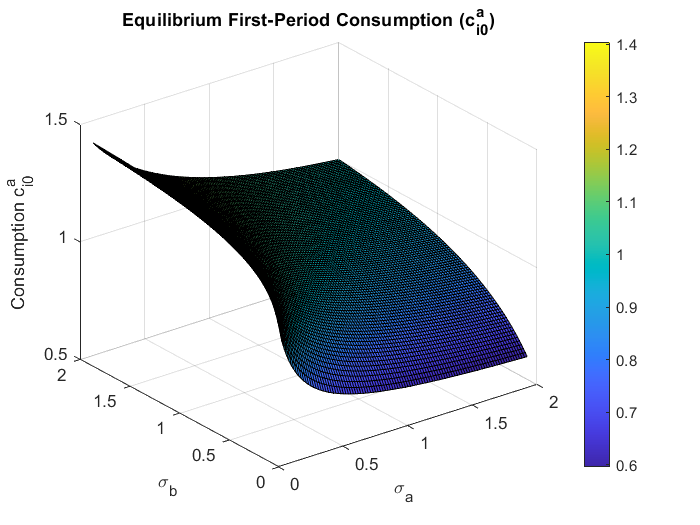
\includegraphics[width=\textwidth]{2b.png}
        \caption{Equilibrium First-Period Consumption $c_{i0}^a$}
        \label{fig:2b}
    \end{minipage}
   % \caption{Bond holdings for types \(a\) and \(b\) as functions of \(\sigma_a\) and \(\sigma_b\).}
    \label{fig:bond_holdings}
\end{figure}

In this problem, agents $a$ and $b$ maximize utility across two periods, trading off present and future consumption. The agents adhere to {Euler equations}, which balance marginal utilities across periods. 
The equilibrium requires solving 1) the {Euler equations for both agents:}
    \[
    (c_{i0}^a)^{-\sigma_a} = \beta (1 + r) \cdot \left[ y_1 + (y_0 - c_{i0}^a)(1 + r) \right]^{-\sigma_a},
    \]
    \[
    (c_{i0}^b)^{-\sigma_b} = \beta (1 + r) \cdot \left[ y_1 + (y_0 - c_{i0}^b)(1 + r) \right]^{-\sigma_b}.
    \]
and 2) the {Market-clearing condition:}
    \[
    c_{i0}^a + c_{i0}^b = 2y_0.
    \]
Agent $a$ maximizes utility, equating marginal utility of first-period consumption with the discounted utility of second-period consumption:
\[
(c_{i0}^a)^{-\sigma_a} = \beta (1 + r) \cdot \left[ y_1 + (y_0 - c_{i0}^a)(1 + r) \right]^{-\sigma_a}.
\]
Agent $b$ behaves similarly, but $c_{i0}^b$ is related to $c_{i0}^a$ through market-clearing:
\[
c_{i0}^b = 2y_0 - c_{i0}^a.
\]
Substituting into agent $b$’s Euler equation gives:
\[
(2y_0 - c_{i0}^a)^{-\sigma_b} = \beta (1 + r) \cdot \left[ y_1 + (y_0 - (2y_0 - c_{i0}^a))(1 + r) \right]^{-\sigma_b}.
\]
The total endowment is divided between agents, ensuring:
\[
b_i^a + b_i^b = 0 \quad \implies \quad c_{i0}^a + c_{i0}^b = 2y_0.
\]

We then demonstrate the numerical solution. 
The system consists of two nonlinear equations:
\[
\text{Equation 1: } (c_{i0}^a)^{-\sigma_a} = \beta (1 + r) \cdot \left[ y_1 + (y_0 - c_{i0}^a)(1 + r) \right]^{-\sigma_a}.
\]
\[
\text{Equation 2: } (2y_0 - c_{i0}^a)^{-\sigma_b} = \beta (1 + r) \cdot \left[ y_1 + (y_0 - (2y_0 - c_{i0}^a))(1 + r) \right]^{-\sigma_b}.
\]

{Numerical solution} is found in the file \verb!macs_pset1_2b.m!
\begin{itemize}
    \item The MATLAB code uses \texttt{fsolve} to solve the system for $c_{i0}^a$ and $r$ iteratively.
    \item The code iterates over a grid of $\sigma_a$ and $\sigma_b$, spanning evenly spaced values between $0.1$ and $2$.
    \item Initial guesses for $c_{i0}^a$ and $r$ are $0.5$ and $0.05$, respectively.
\end{itemize}

The interpretation of these results is then given by the following: 

The first plot shows how the equilibrium interest rate $r$ changes as a function of $\sigma_a$ (risk aversion of Agent $a$) and $\sigma_b$ (risk aversion of Agent $b$). We are familiar with this graph. 

The second plot illustrates how the first-period consumption of Agent $a$ ($c_{i0}^a$) varies with $\sigma_a$ and $\sigma_b$. From the graph and data:
\begin{itemize}
    \item $c_{i0}^a$ decreases as $\sigma_a$ increases.
    \item When $\sigma_b$ is small, $c_{i0}^a$ increases slightly, indicating that Agent $b$ consumes less in the first period, allowing Agent $a$ to consume more.
    \item The highest consumption levels for $c_{i0}^a$ occur at low $\sigma_a$, while the lowest values occur at high $\sigma_a$.
\end{itemize}
The economic implications of this are given by: 
\begin{itemize}
    \item An increase in $\sigma_a$ (higher risk aversion for Agent $a$) leads Agent $a$ to reduce first-period consumption to save more for future periods.
    \item Conversely, when $\sigma_b$ is small, Agent $b$ is less inclined to save, freeing up resources for Agent $a$ to consume more.
\end{itemize}

Interpretations of the Joint Dependence of $r$ and $c_{i0}^a$:
\begin{itemize}
    \item The results from the CSV file and plots reveal a clear inverse relationship between $c_{i0}^a$ and $r$. When $r$ increases due to high $\sigma_a$ or $\sigma_b$, $c_{i0}^a$ decreases as Agent $a$ shifts consumption to future periods.
    \item This relationship reflects the market-clearing condition: higher interest rates incentivize savings and discourage borrowing, leading to a reallocation of resources across periods.
\end{itemize}




%%%%%%%%%%%%%%%%%

\bigskip
    
    \item[(c)] Assume now that \(y_0 = 1\). For the same combination of \(\sigma_a, \sigma_b\) as before, plot bonds \(b_a\) and \(b_b\). Explain the intuition of your results. (20 points)

    \textbf{Solution}

    Solution code can be found at \url{macs_pset1_2c.m}.

\begin{figure}[h!]
    \centering
    % First image for Type a
        \centering
        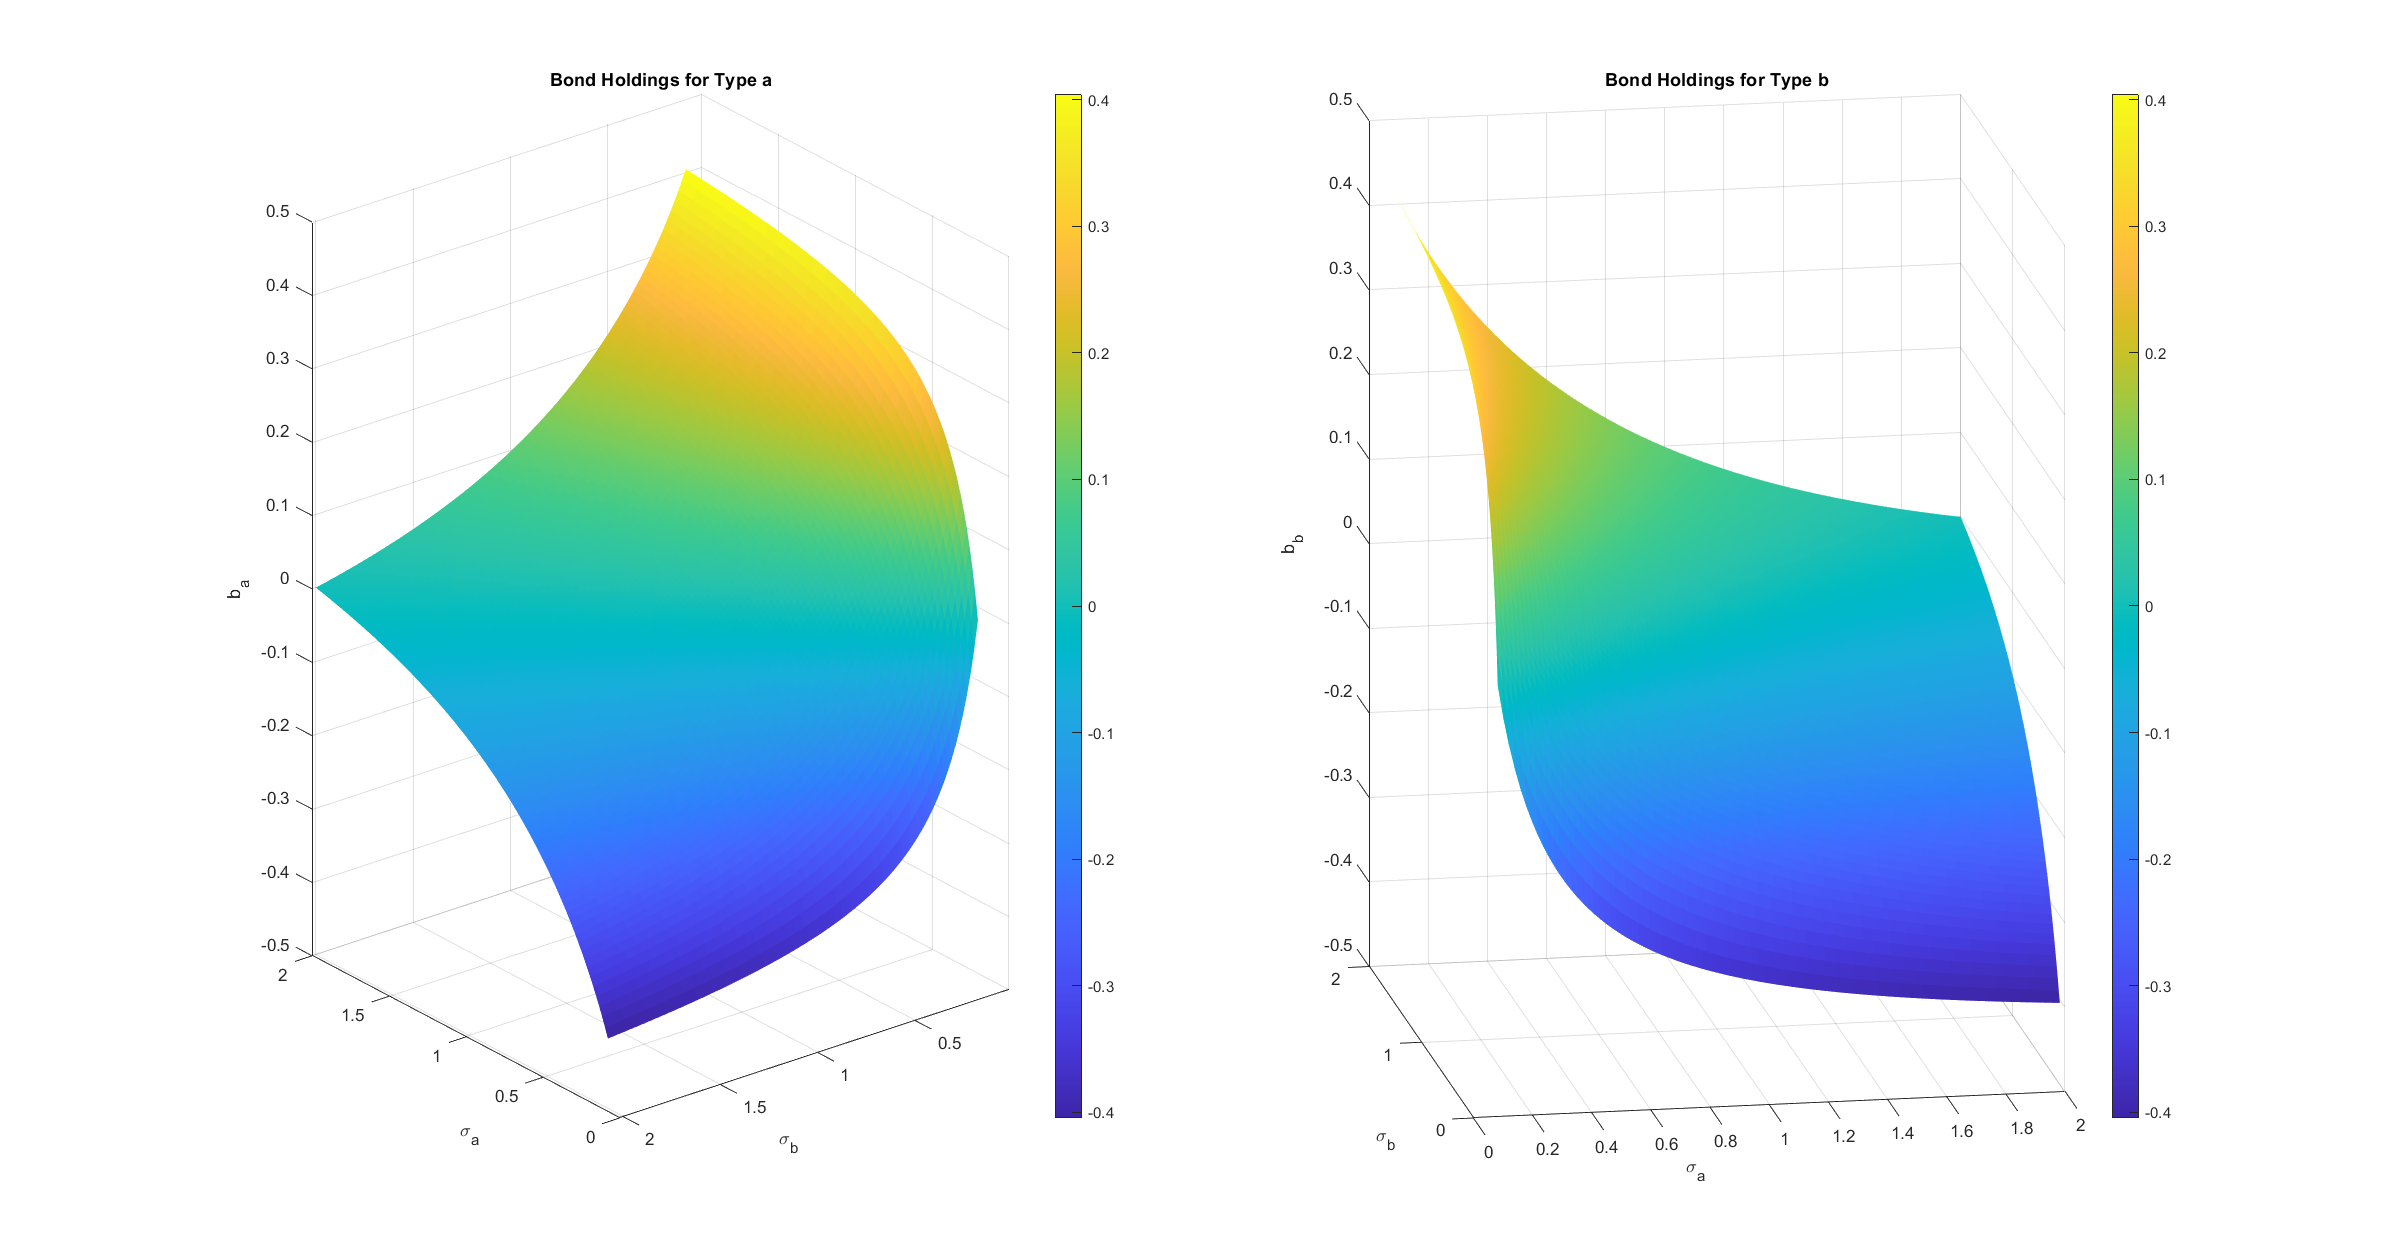
\includegraphics[width=\textwidth]{2c.png}
       \caption{Bond Holdings for Type \(a,b\).}
        \label{fig:bond_a}
\end{figure}


The provided plots show the bond holdings for type \(a\) (\(b_a\)) and type \(b\) (\(b_b\)) households as functions of the risk aversion parameters \(\sigma_a\) and \(\sigma_b\). Below is an interpretation of these results.

\begin{enumerate}
    \item %Type \(a\) Bond Holdings (\(b_a\))
 The plot for \(b_a\) shows a wide range of bond holdings, with values varying from negative to positive depending on the combination of \(\sigma_a\) and \(\sigma_b\).
   When \(\sigma_a\) is low (low risk aversion), type \(a\) individuals are more willing to borrow (negative \(b_a\)).
    As \(\sigma_a\) increases (higher risk aversion), type \(a\) individuals reduce borrowing or even switch to saving (positive \(b_a\)) to smooth their consumption over time.
    The influence of \(\sigma_b\) is also noticeable: higher \(\sigma_b\) (greater risk aversion for type \(b\)) tends to reduce the borrowing of type \(a\), as type \(b\) individuals save more and make funds available in the market.

    \item %**Type \(b\) Bond Holdings (\(b_b\)):**
    The plot for \(b_b\) mirrors the behavior of \(b_a\) but with opposite signs, due to the market-clearing condition \(b_a + b_b = 0\).
    When \(\sigma_b\) is low, type \(b\) individuals are more willing to borrow (negative \(b_b\)).
   As \(\sigma_b\) increases, type \(b\) individuals shift toward saving (positive \(b_b\)), leading to an increase in the availability of funds for type \(a\).

\item % **Symmetry in Market Clearing:**
   The symmetry between \(b_a\) and \(b_b\) reflects the bond market clearing condition:
     \[
     b_a + b_b = 0.
     \]
    When type \(a\) borrows, type \(b\) saves, and vice versa.
\end{enumerate}
 
There are several economic implications from these graphs 
\begin{enumerate}
 \item  % **Impact of Risk Aversion (\(\sigma_a, \sigma_b\)):**
    Higher risk aversion (\(\sigma\)) reduces an individual's willingness to borrow because they place greater value on smoothing consumption over time.
    Conversely, lower risk aversion encourages borrowing to increase immediate consumption.

 \item% **Interplay Between Groups:**
    The bond market connects the two groups. When type \(a\) individuals save more (e.g., due to higher \(\sigma_a\)), type \(b\) individuals borrow less (or save more) because the equilibrium interest rate adjusts to balance the supply and demand for funds.
 \item% **Interest Rate Mechanism:**
    The interest rate \(r\) adjusts to ensure equilibrium. As one group becomes more risk-averse and saves more, the increased supply of savings lowers \(r\), incentivizing the other group to borrow more.

 \item % **First-Period Endowment (\(y_0 = 1\)):**
    The choice of \(y_0 = 1\) ensures that the first-period endowment is symmetric and normalized. This makes the observed variations in bond holdings entirely due to differences in preferences (\(\sigma_a\) and \(\sigma_b\)) rather than differences in initial endowments.
\end{enumerate}


\end{enumerate}

\section*{Problem 3: The Neoclassical Growth Model (30 points)}

In class, we have seen that the Neoclassical Growth Model (NGM) with finite time and inelastic labor supply delivers the following second-order difference equation:
\[
u'(f(k_t) - k_{t+1}) = \beta u'(f(k_{t+1}) - k_{t+2}) f'(k_{t+1}), \quad t = 0, 1, \ldots, T-1,
\]
with \(k_0 > 0, k_{T+1} = 0\). Let the utility function be of the CRRA type:
\[
u(c_t) = \frac{c_t^{1-\sigma}}{1-\sigma}, \quad \sigma > 0,
\]
and the production function:
\[
F(k_t, n_t) = k_t^\alpha n_t^{1-\alpha}, \quad 0 < \alpha < 1.
\]
Recall:
\[
f(k_t) = k_t^\alpha + (1-\delta)k_t.
\]
Consider \(T = 100\) and assume that \(k_0 = 0.1\).

\begin{enumerate}
    \item[(a)] Assume that \(\sigma = 2, \alpha = 0.36, \beta = 0.98\), and \(\delta = 0.025\). Solve the model using a non-linear equation solver. (20 points)

    \textbf{Solution}

    The solved model is found in figure \eqref{fig:3a} from MATLAB code \verb!macs_pset1_3a.m!.

    \begin{figure}[h!]
    \centering
        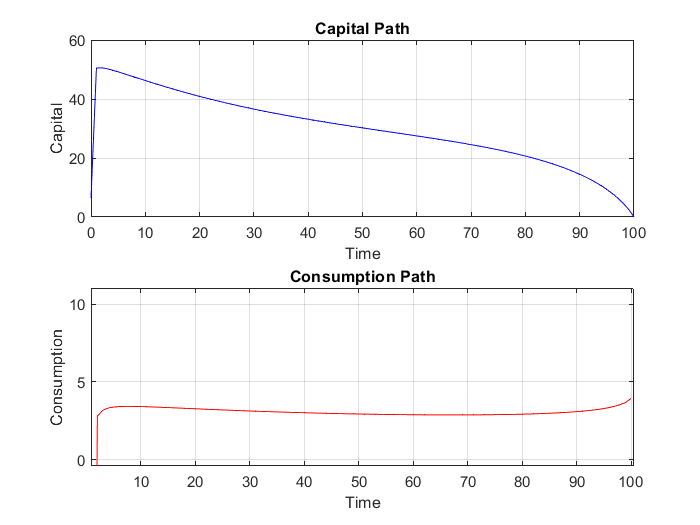
\includegraphics[width=\textwidth]{3a.png}
        \caption{Capital Path and Consumption Path for Problem 3 (a).}
        \label{fig:3a}
\end{figure}

    \item[(b)] Assume now that \(\sigma = 1, \alpha = 0.36, \beta = 0.98\), and \(\delta = 1\). Solve the model using a non-linear equation solver. Show that the solution is the same as that given by the analytical solution for this case. (10 points)

    \textbf{Solution}

    The solved model is found in figure \eqref{fig:3b} from MATLAB code  \url{macs_pset1_3b.m}.

    \begin{figure}[h!]
    \centering
        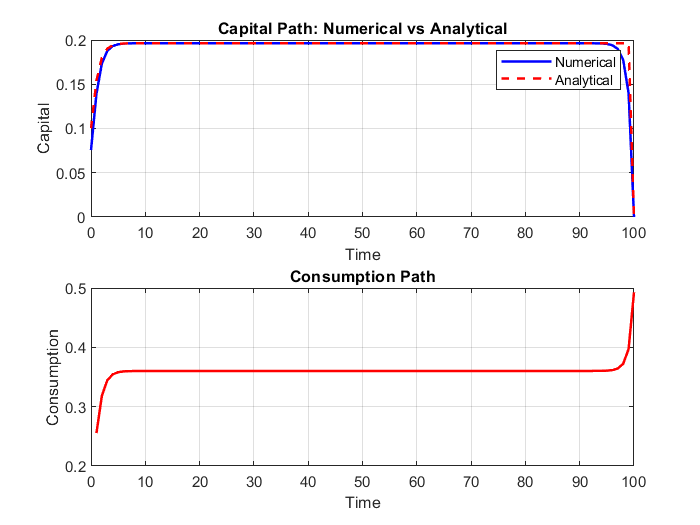
\includegraphics[width=\textwidth]{3b.png}
        \caption{Capital Path and Consumption Path for Problem 3 (b).}
        \label{fig:3b}
\end{figure}
    
\end{enumerate}

\end{document}

